\section{What is machine learning} \label{ch:what_is_ml}

\subsection{Machine learning in general}

Usually programming consists of applying rules to certain problems to get solutions.
By using machine learning we want to build a model which uses
solutions to certain problem to figure out the respective rules \footnote{ TODO }.
% TODO: Add figure of François Chollet here. Maybe use a citation here?

The promise made by machine learning is that the rules learned can be significantly more
complex than it is feasible to program them by hand.
A good example for this is image recognition (which will be the focus of this project),
in which the content of images is to be classified. Relations between pixels have to be
figured out resulting in a complex model. This is not feasible to program in traditional
manner even for the simplest tasks.

The algorithm trained to fulfil the task at hand is called the model.
The model inherits the hypothesis which states that for a function $h$ there is a
mapping of input $x$ to the correct output $y$ via a parameter tensor \theta.
This notion is summarized in equation~\eqref{eq:hypothesis}.

\begin{equation} \label{eq:hypothesis}
\exists \theta \in X . \forall x \in I . h_\theta(x) = y(x)
\end{equation}

The hypothesis can be thought of as an n-dimensional polynomial function.
For model evaluation a loss function is used;
it compares the result of the hypothesis with provided data.
The lower the loss the better the model is performing on a given input.
The loss function is defined through an equation like equation~\eqref{eq:loss}
in the form of a sum, taking some measurement
of the deviation of the actual state to the desired state.

\begin{equation} \label{eq:loss}
L(\theta) = \frac{1}{m} \sum_{i=1}^m L_i(\theta)
\end{equation}

For the loss function to gradually decrease, $\theta$ is iteratively adjusted using an
optimizer function which is famously done using gradient descent or some variant of it (which will
be further examined in chapter~\ref{ TODO }).
Gradient descent is performed by calculating the gradient of the loss function and subtracting it
from the respective parameters, shown in equation~\eqref{eq:gradient_descent}.

\begin{equation} \label{eq:gradient_descent}
\theta_{i+1} = \theta_i - \eta \nabla_\theta L(\theta)
\end{equation}

Herein $L$ is the loss function and $\eta$ is a learning rate which will be discussed in
chapter~\ref{ch:over_and_underfitting}.

If equation~\eqref{eq:hypothesis} holds to be true the model is therefore going to be a sufficient
fit for the given input. Subsequently these concepts are introduced using a simple example.

\subsection{Simple linear example} \label{ch:simple_linear_example} % TODO more descriptive title?

As an illustrative example a model translating Fahrenheit into Celsius will be created.
The original equation is given by the linear function $y = mx + b$
as $F = C * 1.8 + 32$, with $F$ as degree Fahrenheit and $C$ as degree Celsius
respectively.

A model designed to learn this relationship is defined in listing~\ref{lst:c_to_f}.

% TODO add JavaScript as language
\lstinputlisting[label={lst:c_to_f}, caption={Celsius to Fahrenheit}]{demos/c_to_f.js}

The model described has the properties
\code{m}, \code{b} (from $mx + b$) and the hypothesis representing the linear relationship.

\code{y} provides the correct answer. Please note that \code{y} is only used in training
and can be omitted once the model parameters are properly adjusted.

In this example the loss function is described by the \textit{mean squared error }
\footnote{ Abbreviated as \textit{mse} } which is shown in equation~\eqref{eq:mse}.

\begin{equation} \label{eq:mse}
L = \frac{1}{2 m} \sum_{i=1}^{m} (h_\theta(x_i) - y(x_i))^2
\end{equation}

Whereas $L$ is the value of the loss, $m$ is the sample size, $h$ is
the hypothesis and $y$ is the validation function.
The input tensor $\theta$ contains all parameters of the hypothesis;
$\theta_0$ traditionally representing the bias node\footnote{ TODO }.

To minimize the loss function gradient descent described in equation~\eqref{eq:gradient_descent}
is used.

In listing~\ref{lst:c_to_f} equation~\eqref{eq:gradient_descent} is implemented as \code{sgd} using
$\theta_0 = \code{b}$ and $\theta_1= \code{m}$ as shown in equation~\eqref{eq:sgd_mse_here}.

\code{sgd} is short for\textit{stochastic gradient descent}.
\footnote{A distinction is made between batch, mini-batch and stochastic gradient descent;
using the full data set, a defined subset or single inputs respectively on each iteration.}
It represents the optimizer function, updating the
parameters of the model by taking the gradient of the loss for each individual parameter and
updating them simultaneously.

\begin{equation} \label{eq:sgd_mse_here}
\begin{split}
m_{i+1} & = m_i - \frac{\partial L}{\partial m_i} = m_i - (h(x) - y(x)) * x \\
b_{i+1} & = b_i - \frac{\partial L}{\partial b_i} = b_i - (h(x) - y(x))
\end{split}
\end{equation}

The respective output may look like:
\begin{lstlisting}
loss:  343041.666256673
loss:  16242.7707476548
loss:  88.27595280422442
loss:  10.74432403839251
loss:  1.1607137779951606
loss:  0.252186283500194
loss:  0.00040450626910586374
loss:  0.00004247033303206121
loss:  7.158429555712516e-7
loss:  1.6948019668728757e-10
weights:  [ 31.99999973758735, 1.8000003977458756 ]
\end{lstlisting}

Expected behaviour for the loss function is to decrease, which it evidently
does and thereby showing that the deviation of the hypothesis to the actual result is diminishing.
After iterating 200 times the parameters \code{m} and \code{b} of the \code{model} are logged
and show that they are actually close to the expected result.
By increasing the iteration count, the result can be increased to the point where they are rounded
to represent exact results (using Node.js\footnote{ TODO }).

\begin{SCfigure}
    \centering
    \caption{ The provided example may be visualized like this. The bias can be interpreted as
    an extra input which is always 1. The input is multiplied by the parameters
    labelling their respective arrows, which are in turn summed up
    (resulting in $y = mx + b$) }
    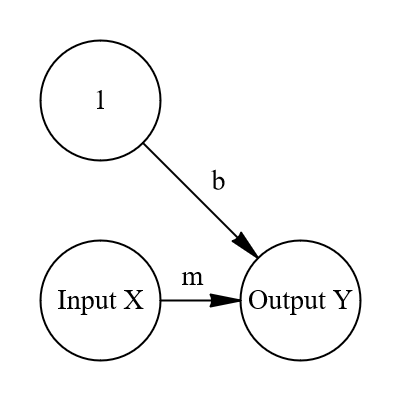
\includegraphics[width=0.4\textwidth]{images/1_simplest_nn.png}
    % \label{fig:nn1}
\end{SCfigure}

The code can be found under
\url{https:// klawr.github.io/deepmech/reports/srp/demos/c_to_f.js}
and can be executed using Node.js.


Provided this hypothesis is initially well suited for the task, it is important to note
that by modify the hypothesis to represent a polynomial of a higher degree
(e.g. $y = nx^2 + mx + b$) the extra parameters are converging to zero,
effectively providing the same result as before
\footnote{But to achieve similar results the iteration count has to be increased by at least a
factor of 20. You can review the experiment under
\url{https://klawr.github.io/deepmech/reports/srp/demos/c_to_f_adv.js}}.

\subsection{Neural Networks} \label{ch:neural_networks}

To extend the output to more nodes,
thus creating the context necessary for tasks with multiple outputs, a more complex structure
is required; introducing neural networks, which is very
prevalent in the deep learning context.

Despite the name neural networks being neither neural, nor networks\footnote{ TODO },
the name is now generally accepted due to historical reasons; initially having the
brain as inspiration\footnote{ TODO } they are used to create are more complex mapping 
of input to output.

% TODO heavily citations necessary here...
Neural networks allow for more complicated relationships between nodes of different layers,
introducing hidden layers between the input and the output.
Furthermore even though the universal approximation theorem states that all continuous function
can be described using only one hidden layer, in practice it is much more feasible to
add hidden layers, thus increasing the size of the neural network linearly with the feature size,
instead of exponentially\footnote{Even though the exact structure is a topic on its own and is
discussed in chapter~\ref{ TODO }}.

Adding hidden layers to the model, neural networks are hence called deep neural networks (DNN)
and the training of those models is congruently called deep learning.
The loss function $L$ does not change in the dilation of the model to a neural network;
however the previous equation~\eqref{eq:gradient_descent} does not suffice updating all
parameters in all layers, since it only considers updating the elements of the last layer.
The last layer however is itself a function of the previous layer, and that layer is again
a function of the previous layer and so on. Going backwards in this manner, the chain rule can be
applied to the model. This process is fittingly called
backpropagation\footnote{Short for "backward propagation of errors"\ref{ TODO }} and described in
equation~\eqref{eq:backpropagation}.

% TODO this is utterly crap and should be corrected...
\begin{equation} \label{eq:backpropagation}
\theta_{i+1, j}^k = \theta_{ij}^k - \eta \nabla_\theta L
\end{equation}

Another common method to be used in neural networks are activation functions.
Activation functions take an input and apply some modification or normalization
to this input. In practice it is established that some form of activation functions
increase the stability of the overall model.
Popular activation functions are the sigmoid and the ReLU-function both described in
equation~\eqref{eq:sigmoid_relu}\footnote{If no activation is used it is called linear
activation hence $f(x) = x$ is technically valid}.

\begin{equation} \label{sigmoid_relu}
\begin{split}
Sigmoid: f(x) & = \frac{1}{1 + \exp^{-x}} \\
ReLU   : f(x) & = max(0, x)
\end{split}
\end{equation}

Keeping that in mind the
backpropagation algorithm has to be extended by another layer of derivation using the
chain rule described in equation~\eqref{chain_rule_for_activation}.

\begin{equation} \label{chain_rule_for_activation}
\nabla_{\theta^k} L = \frac{\partial L}{\partial \theta_{ij}^k} =
\frac{\partial L}{\partial a_{ij}^k} \frac{\partial a_{ij}^k}{\partial \theta_{ij}^k}
\end{equation}

% TODO Overfitting and underfitting -> Generalization

% TODO introduce AND, OR, XOR gates here